\section{Public key cryptography}

Public key cryptography is the backbone of most distributed systems as it provides both a way to encrypt a message as to validate the source of a message, without the need to agree upon a shared key. The most used implementation of this idea is the RSA encryption method, named after inventors Rivest, Shamir and Adleman \cite{rsa-patent}. 

\subsection{Basics}

In previous encryption systems before the public key cryptography, two parties who wanted to safely exchange messages needed to agree on a common cypher first. One of the more famous of such encryption systems is the Ceasar cypher \cite{ceasar-cypher}, in which the cypher consisted of offsetting every character with a previously agreed upon number. However, if a third party manages to intercept transmission of this cypher itself, all encrypted messages can easily be decoded. Therefore, a trusted third party network is needed to securely exchange the cypher.

Public key cryptography uses a pair of hashes instead. These hashes are often referred to as the keys. These hashes are algorithmically generated so that they are cryptographically connected: data encrypted with one key can only be decrypted with the other key and visa versa \cite{rsa-paper-explanation}.

One of these keys can be publicly broadcasted. As a result, everyone knows that this key is connected to the owner's identity. Therefore, it is referred to as the public key.

The other key will be held privately. It is very important that nobody except the owner know the content of this key, as it will be used to prove the owner's identity. It is therefore referred to as the private key.

Because no cypher has to be exchanged, there is no need for the trusted middleman to exchange the cypher, eliminating a key weakness of cypher encryption.

\subsection{Uses: encryption and source validation}

A first use case of public key cryptography is encryption. If a person called Alice wants to send a message to Bob, she encrypts her message with Bob's public key. As a result, only Bob  can decrypt this message as only Bob knows the corresponding private key. The message can now be send over any insecure network, such as the internet, email or even carrier pigeon, without any danger of leaking its contents.

Besides encryption, public key cryptography can also be used for source validation. If Alice wants to broadcast a message to the world, she can encrypt the message with her private key. As the encrypted message can only be decrypted with Alice's public key, everyone knows that only Alice could have encrypted it. This case is often referred to as a digital signature, as Alice signed the message with her private key. 

For full security, a secure message is often first encrypted with the private key of the sender and then the public key of the recipient. Now only the recipient can decrypt the message and can then validate the origin of the message. This full process is modeled in figure \ref{fig:rsa-diagram}.

\begin{figure}[h]
\centering
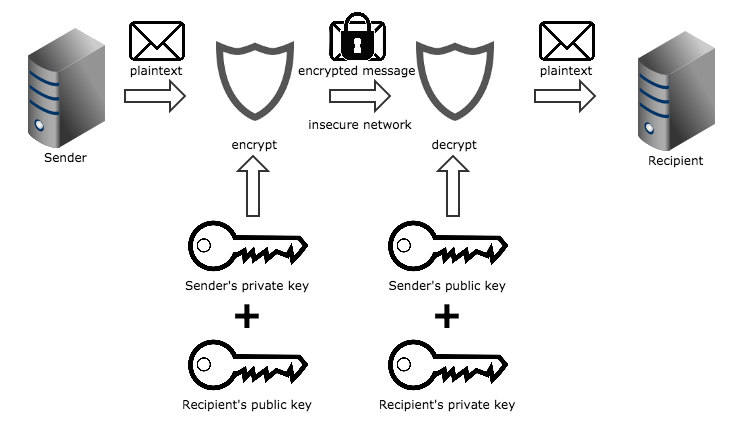
\includegraphics[width=0.8\textwidth]{paper-images/rsa-diagram.png}
\caption{}
\label{fig:rsa-diagram}
\end{figure}

